\documentclass[11pt,twoside]{report}
\usepackage{preamble}
\graphicspath{{../img/ch5/}}
\setcounter{chapter}{5}


\begin{document}

\chapter{Analysing The Zebrafish Behaviour}
\label{chapter:fish_analysis}


\section{Introduction}


Some descriptive quantities such as density distribution, average speed, and degree of polarisation would also be presented. Inspired by the soft--matter community, I also calculated the temporal and spatial correlation functions to characterise the system. These quantities and correlation functions will serve as the final target for modelling the zebrafish in the next chapter.


\section{From Locations to Trajectories}


\subsection{Removing Overlapped Particles}
\label{section:overlap}

I used linear programming method to remove overlapped coordinates. The overlap happened if different parts of the fish matched different kernels.

Supposing there are $N$ particles in total, and we wish to find $K$ non--overlapping particles, where each particle has an uncertainty value of $e_i$. The task can be written as a linear programming problem with quadratic constrains as follows:

\begin{equation}
\begin{aligned}
	\textrm{Minimize} && \sum_i{e_i x_i} \\
	\textrm{Subject to} && d_{12} x_1 x_2 \le \sigma \\
	&& d_{13} x_1 x_3 \le \sigma \\
	&& \vdots  \\
	&& d_{ij} x_i x_j \le \sigma \\
	&& \sum_i{x_i} = K
\end{aligned}
\end{equation}

\noindent where $d_{ij}$ is the distance between particle $i$ and $j$, $\sigma$ is the diameter of the non--overlapping hard core of each particle, and $K$ is the total number of particles. The solution to above cost function and constrains can be effectively solved by the CPLEX optimisation package. (SITE IBM).\marginfootnote{As a recent development, IBM announced a faster version of CPLEX using the deep neural network to perform the same optimisation task.}

An alternative choice is to apply a greedy algorithm, to always remove the worst match until there is no overlap. The greedy algorithm is much easier to implement, and can sometimes find good solutions. However, the linear programming method will find the global minimum of the cost, therefore being selected in my study.

The overlapping resolve method introduced in this subsection can be extended beyond tracking animals. In fact, it can be very helpful to refine the particle tracking result for colloidal experiments, where the traditional algorithm might give overlapping coordinates because of intensity noises. In the colloidal experiment, the error term can be the inverse of the fluorescent intensity (to favour brighter centres) or the response to a kernel function (to favour a particular shape).

\subsection{Linking Positions to Trajectories}
\label{section:link}

With the positions of all the fish, one can study the \emph{structure} of the fish group. However, extra work needed to be carried out in order to obtain the \emph{dynamic} of the system. Because the velocities of each fish is needed to calculate the dynamical quantities like the spatial/temporal velocity correlation function, which is used to extract the correlation length and the leadership relationship. To get the velocities, it is necessary to link the positions, at different time points, into trajectories. The concept is illustrated in.

% words and figure to illustrate a linking procedure.

The linking procedure requires a prior knowledge of the dynamic of the system under study. For example, the dynamic of colloidal particles is known to be Brownian, whose.

% introduce the CG linking procedure.

However, the situation for the fish is a bit different: we don't really know the dynamic of the fish, hence the cost function to minimise in the linking procedure is a bit unclear.

To tackle the situation, to my best knowledge, one can start with very simple assumptions. One possible choice is the constant speed.

% introduce Ouellette's paper.

Implementing the algorithm, I obtained some very short trajectory segments. These segments can be extended further following

% introduce Xu's idea and the global optimisation procedure.

Practically, enumerating all the possible linking choices can take a very long time. So

% talk about the heuristic to restrain dt dx.

Pass



\subsection{Analysing the Trajectories}

Several quantities were calculated to analyse the trajectories of the fish, and the calculations are generic for both 2D and 3D trajectories. Therefore these quantities will also be used in Chapter~\ref{chapter:fish_3d}.

\begin{SCtable}
	\begin{minipage}[b]{\linewidth}
	\centering
		\begin{tabular}{c l c r}
			\toprule
		    Symbol & Name & Unit & Comment \\
		    \midrule
		    $v_0$ & Speed & mm/s & Average over different fish\\
		    {\dnn} & Nearest Neighbour Distance & mm & Average over different fish\\
		    $\Phi$ & Polarisation &  1 & Larger = ordered movement\\
		    $\left\langle \cdot \right\rangle$ & Average operator  & &  Time average\\
		    {\mtau} & Relaxation time & s & The relax of fish orientation \\
		    {\meps} & Effective Attraction & 1 & Smaller = more cohesive\\
		    {\mlp} & Persistence Length & mm & Defined as {\mspd}{\mtau} \\
		    $\kappa$ & Reduced Persistence Length & 1 & Defined as {\mlp} / {\mdnn} \\
		    \bottomrule
		\end{tabular}
	\end{minipage}
	\label{tab:behaviour-quantities}
	\caption{A summary of the variables used to describe the fish behaviour.}
  \label{table:geometry}
\end{SCtable}


\subsection{Refine the Trajectories}

The 3D positions obtained from the tracking system can be linked into trajectories described in section \ref{section:link}. The linked trajectories are good, thanks to the predictive linking method and the subsequent relinking, but it is still possible to further optimise the trajectories. The idea is to re--incorporate the information of the 2D features and cameras into the trajectories.

\subsection{Accuracy Evaluation}

I evaluated the accuracy of the tracking method with the simulated data. Typically, I generated the trajectories of 50 simulated fish inside a container. Then I use the software \emph{Blender} (version 2.91.0 on Ubuntu 20.04) to render the movement of the fish as animations, with multiple cameras. The result movies looks very similar to my experimental videos, in terms of the local fish density and the speed. This similarity ensured the accuracy that I assessed from the simulation movie is valid for my experimental data.


\section{From Trajectories to Behaviour}

\subsection{The Static Features}

\subsection{The Dynamical Features}


\section{The Behaviour of Zebrafish in 2D}


\section{The Behaviour of Zebrafish in 3D}

The 3D tracking yields the positions of the fish, whose discrete time derivative gives the velocities. From these two quantities, we calculate three global descriptors to characterise the behaviour of the fish: the average speed, the polarisation, and the nearest neighbour distance. The average speed is defined as $v_0 = 1/N \sum{|\vi|}$ where $i$ runs over all the tracked individuals. 

For experiments with more than one fish, the polarisation $\Phi$ was commonly used to characterises the alignment of the velocities. It is defined as the modulus of the average orientation, written as \cite{attanasi2014pcb},
$\Phi = 1/N \left| \sum{({\vi}/{| \vi |}}) \right|$ where $i$ runs over all the individuals. Large polarisation ($\Phi \sim 1$) signifies synchronised and ordered movement, while low polarisation indicates decorrelated, random movement. The polarisation is sometimes referred to as the ``order parameter'' by physicists, since it is a measure of the order of the fish dynamic. We say a group of fish have \emph{ordered} movement if they are swimming towards the same direction.\marginfootnote{If we think of the moving direction of the fish as little spins of a magnetic system, then the polarisation is mathematically equivalent to the average magnetization per spin.}

The local density of the group also plays important roles in the collective behaviour. The local density can be probed by the nearest neighbour distance, which is noted as {\dnn} in this thesis. For a fixed number ($N$) of fish in a fixed sized environment (with volume $V$), their overall number density is constant (being $N/V$). However, the groups with smaller {\dnn} is more cohesive.


\subsection{A Single Fish}
\label{section:fish_1_3d}


Figure~\ref{fig:density_3d_fish_1} shows the spatial distribution of one fish in the observation tank. It is obvious that the fish tend to stay in the bottom of the tank. It is a typical fish behaviour when they were subjected to a new environment, and it is known as the ``depth preference''.
Nevertheless, the distribution of the $X$ components of the coordinates is symmetric, which suggests the fish do not have a preferred location to stay in the tank.


\begin{SCfigure}
  \includegraphics[width=\linewidth,outer]{density-one-fish}
  \caption[The 3D spatial distribution of one fish]{The spatial distribution of one adult zebrafish. The top panel shows the joint distribution of the $Y$ coordinates and $Z$ coordinates of the fish positions. The bottom panel shows the distributions of the $X$ coordinates, the planar radius ($R$) and the $Z$ coordinates. The distribution of the ideal gas in the tank was given as a reference.}
  \label{fig:density_3d_fish_1}
\end{SCfigure}

From the fish trajectories, we can also calculate their speed and orientations in each from. These time series also offer the typical time scale of speed changing and orientation relaxing.


\subsection{A Pair of Fish}
\label{section:fish_2_3d}

The spatial distribution of 2 zebrafish were presented in Fig~\ref{fig:density_3d_fish_2}. The behaviour of 2 fish is similar to that of one fish. Namely, the fish tend to be around the bottom of the tank.

\begin{SCfigure}
  \includegraphics[width=\linewidth,outer]{density-two-fish}
  \caption[The 3D spatial distribution of two fish]{The spatial distribution of two adult zebrafish. The top panel shows the joint distribution of the $Y$ coordinates and $Z$ coordinates of the fish positions. The bottom panel shows the distributions of the $X$ coordinates, the planar radius ($R$) and the $Z$ coordinates. The distribution of the ideal gas in the tank was given as a reference.}
  \label{fig:density_3d_fish_2}
\end{SCfigure}

The fish interaction can be probed by the relative distribution of the neighbours of the fish. 


\subsection{Three Fish}
\label{section:fish_3_3d}

The spatial distribution of 2 zebrafish were presented in Fig~\ref{fig:density_3d_fish_3}. Being similar to the one fish and two-fish case, a group of three fish presents the depth preference.

\begin{SCfigure}
  \includegraphics[width=\linewidth,outer]{density-three-fish}
  \caption[The 3D spatial distribution of three fish]{The spatial distribution of three adult zebrafish. The top panel shows the joint distribution of the $Y$ coordinates and $Z$ coordinates of the fish positions. The bottom panel shows the distributions of the $X$ coordinates, the planar radius ($R$) and the $Z$ coordinates. The distribution of the ideal gas in the tank was given as a reference.}
  \label{fig:density_3d_fish_3}
\end{SCfigure}

\subsection{Many Fish}
\label{section:fish_many_3d}

We studied the behaviour of 50 fish with two different age groups, the {\smallfish} whose age is between 6 months old to 1 year, and the {\bigfish} whose age is beyond 1 year.

The behavioural quantities, as I summarised in Table~1, is shown in Fig~\ref{fig:descriptor-many-fish}.

\begin{SCfigure}
  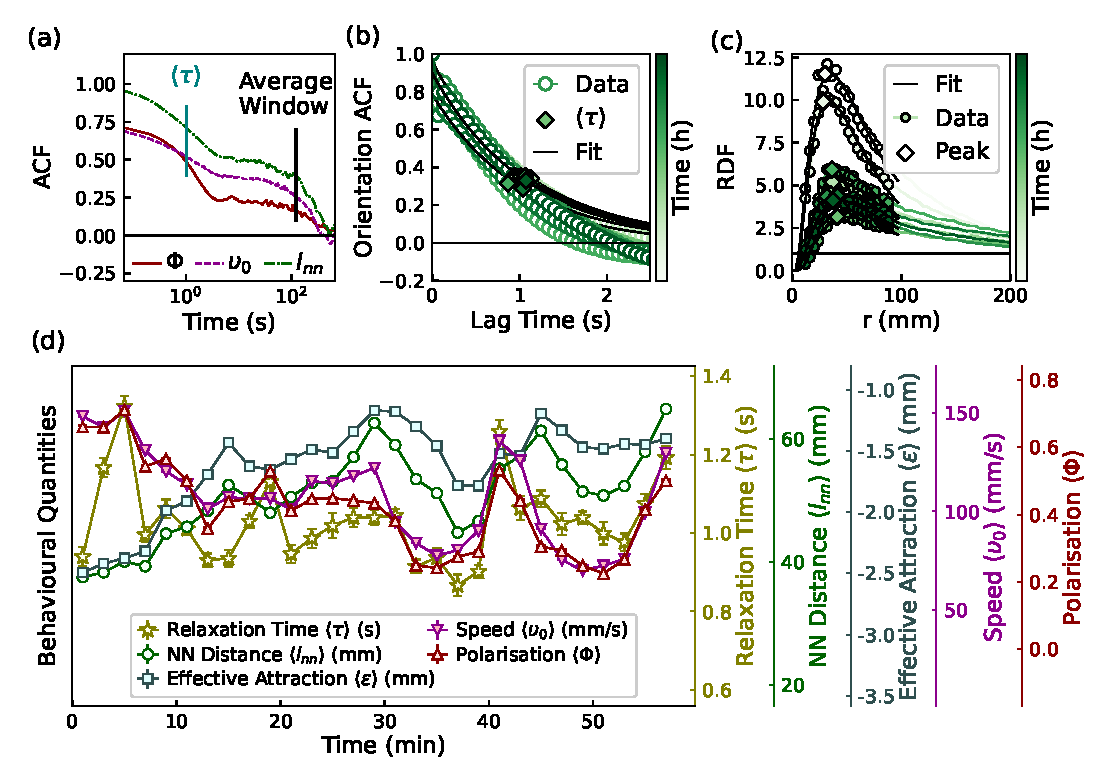
\includegraphics[width=\linewidth,outer]{descriptor-many-fish}
  \caption[The behavioural descriptors of 50 zebrafish]{
  	(a): The auto--correlation function of the polarisation and average speed of the fish group.
	(b): The auto--correlation function of the orientations of fish.
	(c): Sequence of radial distribution functions with increasing time: at early times (top curves) the fish are clustered together so that the peak is large; at later times (bottom curves) the local density decreases and so does the peak height.
	(d): The time evolution of the averaged {\descriptors} for 50 {\smallfish} fish. Each point corresponds to the average value in 2 minutes.
	The error bars illustrate the standard error values.
  }
  \label{fig:descriptor-many-fish}
\end{SCfigure}

\section{Conclusion}

\end{document}
